%\documentclass[10pt,a4paper]{article}
\documentclass[12pt,a4paper]{article}
\usepackage{graphicx,amsmath}
%\usepackage{subfigure}
\usepackage{float}
\usepackage[german]{babel}
\usepackage[utf8]{inputenc}
\setcounter{secnumdepth}{4}
\usepackage[top=2cm, bottom=2.5cm, left=3cm, right=3cm]{geometry}
\usepackage{subcaption}
\begin{document}


%\title{Bachelorarbeit}
%\author{Richard Kullmann}
%\date{02.06.2017}

\thispagestyle{empty}
%\setcounter{page}{2}
\newpage
\tableofcontents
\thispagestyle{empty}
\newpage
\pagenumbering{arabic}

\section{Vergleich SNR-Theorie}
Das Signal-zu-Rausch Verhältnis kann für ein Kosinus-Signal mit Stärke $\epsilon$ folgenderma"sen berechnet werden:
\begin{align*}
SNR=\frac{\epsilon ^2T}{4}\frac{|\chi(\omega)|^2}{S_0(\omega)}=\frac{\epsilon^2T|\chi(\omega)|^2}{8\cdot D_{eff}}
\end{align*}
Wenn man die Ableitung der Feuerrate numerisch aus vorherigen Messungen bestimmt und den gemessenen Diffusionskoeffizienten verwendet, lässt sich eine gute Vorhersage des SNR treffen

\begin{figure}[H]
	\centering
	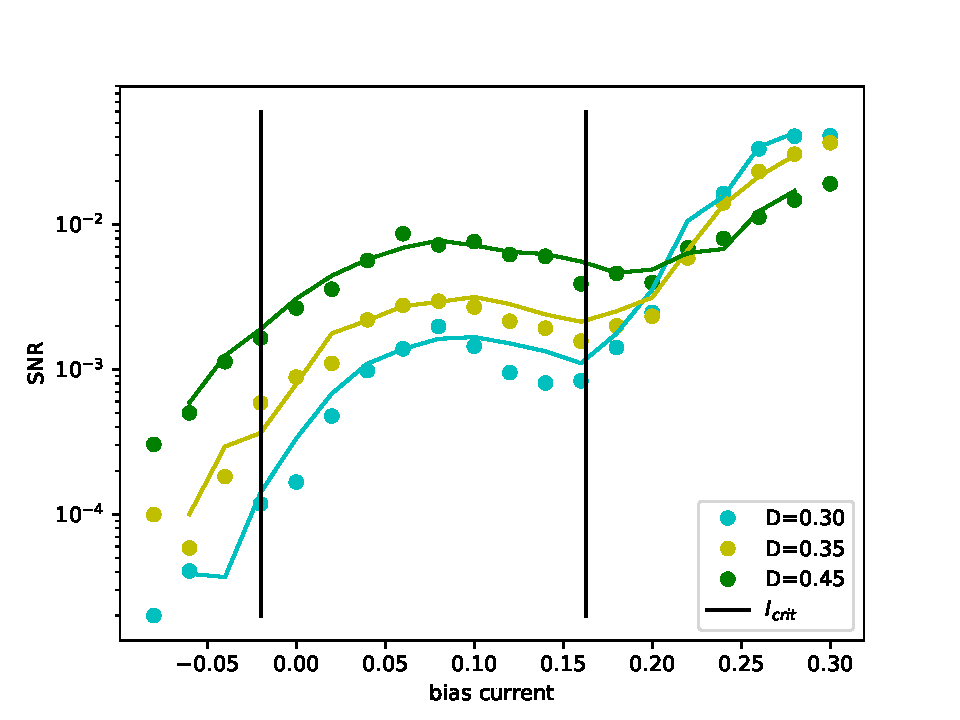
\includegraphics[scale=0.9]{snrangerealanameassp.pdf}
	\caption{Vergleich des SNR mit anderen Messwerten}
	\label{snrspike}
\end{figure}

Die mittleren Feuerraten nähern sich bei zunehmendem Bias-Strom $I$ der mittleren Feuerrate im burstenden Zustand an:
\begin{figure}[H]
	\centering
	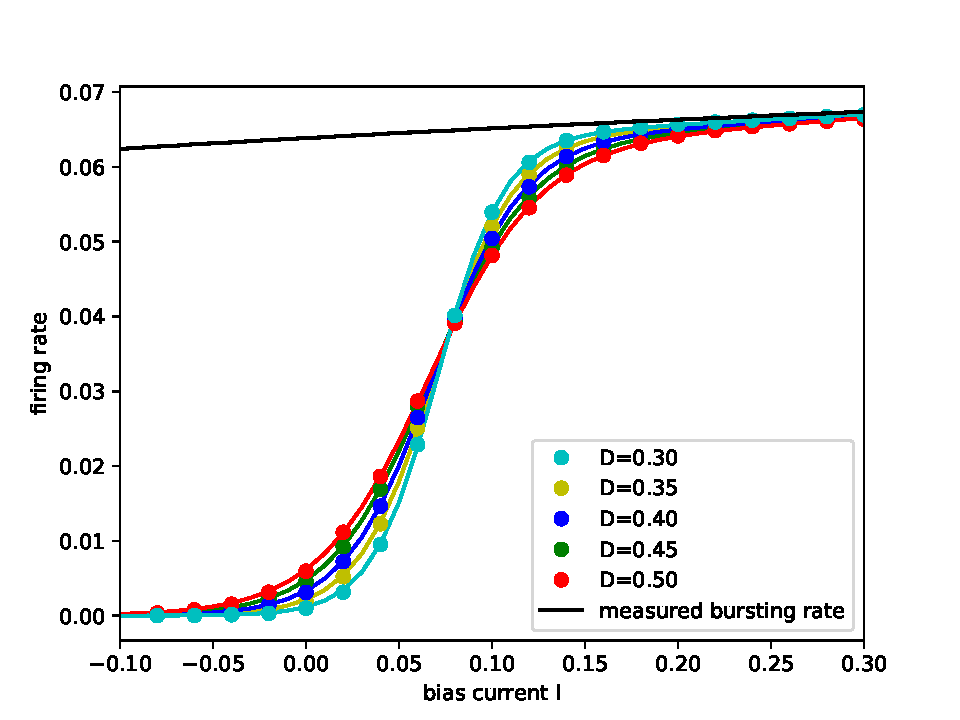
\includegraphics[scale=0.9]{ganaburst.pdf}
	\caption{Feuerraten und entsprechende Fits}
	\label{feuerrate}
\end{figure}

Das SNR des Spike Trains zeigt deutlich ausgeprägter das erwartete Verhalten:

\begin{figure}[H]
	\centering
	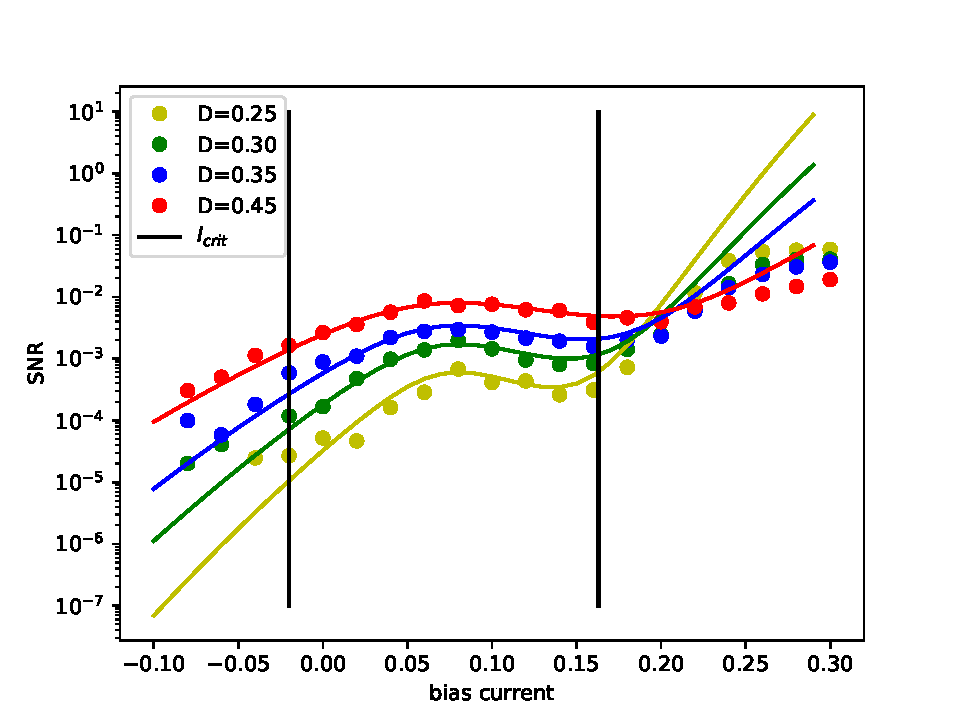
\includegraphics[scale=0.9]{snrautoreal13a25snrsp.pdf}
	\caption{Vergleich theoretisches und gemessenes Spektrum}
	\label{deltaspectrum}
\end{figure}
Es ist jedoch noch kein Zusammenhang mit dem kritischen Strom erkennbar.\\
Im Bereich des kritischen Stroms wurden dementsprechend längere Messungen vorgenommen:
\begin{figure}[H]
	\centering
	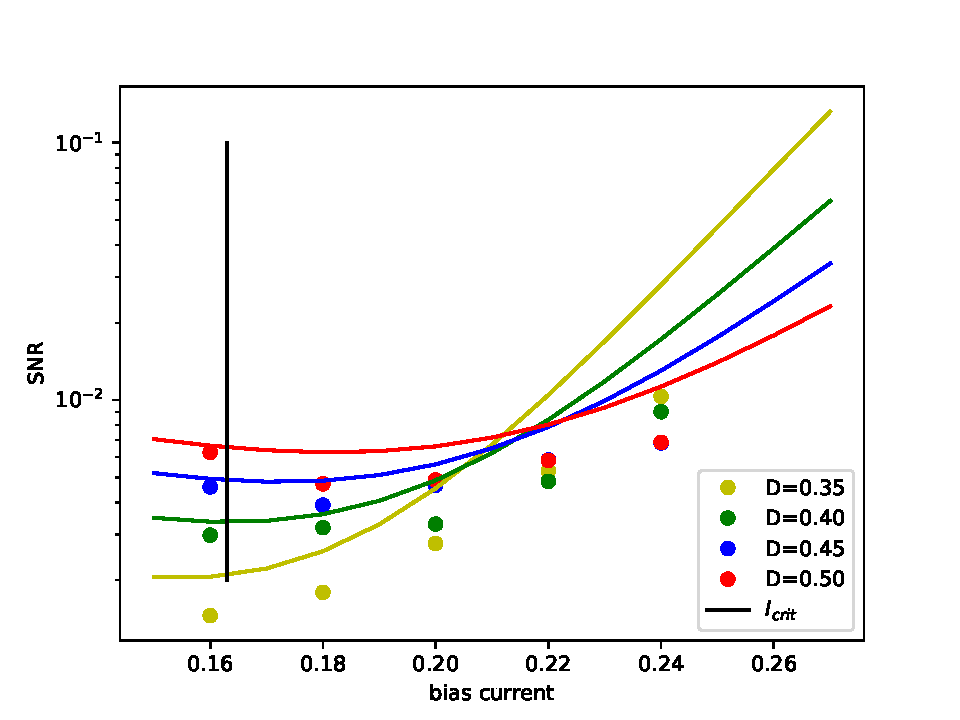
\includegraphics[scale=0.9]{snrpoi31a.pdf}
	\caption{SNR für verschiedene Werte von D}
	\label{drange}
\end{figure}
Es ergibt sich ein Schnittpunkt, der auch in etwa an der Stelle ist, die die Theorie vorhersagt. 
\begin{figure}[H]
	\centering
	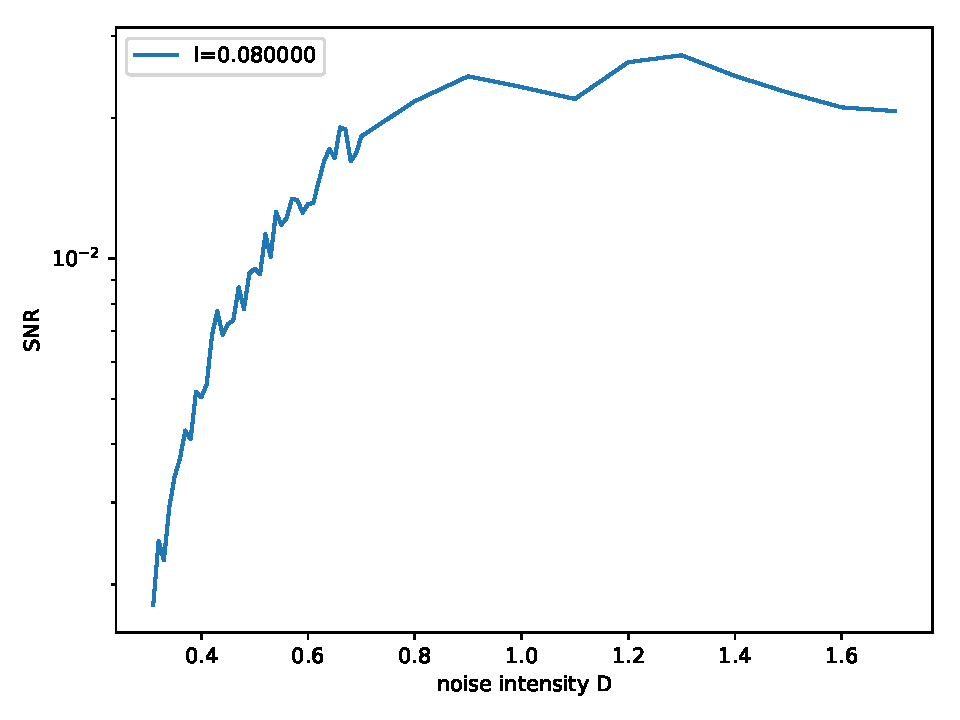
\includegraphics[scale=0.9]{snrautoabglongrealdrange6aem2.pdf}
	\caption{Verhalten des SNR über verschiedene D}
	\label{dcomp}
\end{figure}
Das quadratische Fitten der Potentialbarrieren liefert ein deutlich besseres Ergebnis als der lineare Ansatz:
\begin{figure}[H]
	\centering
	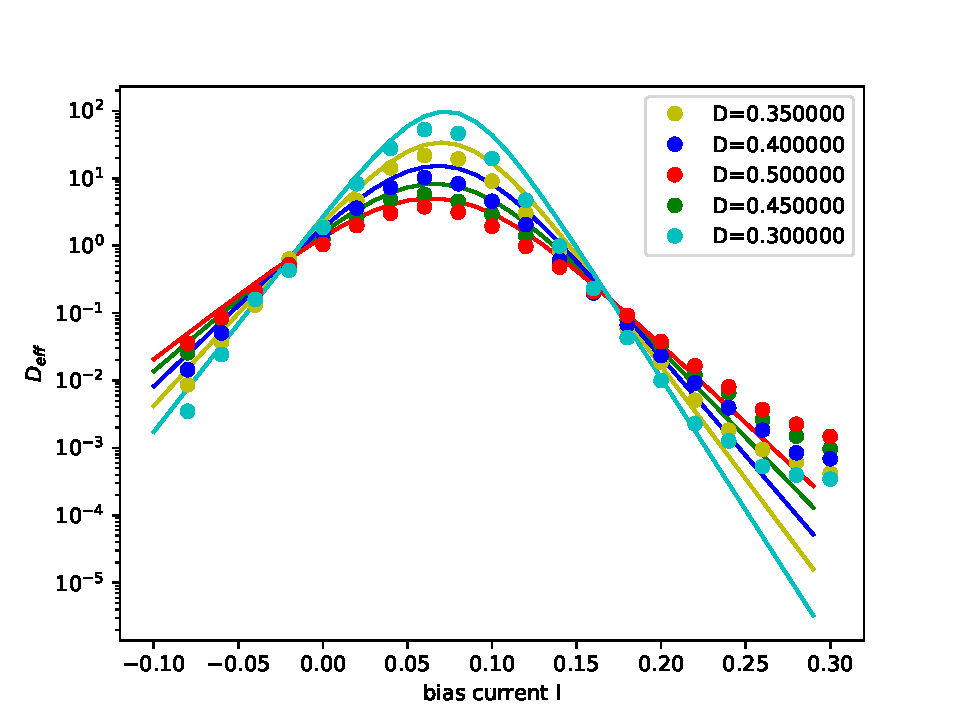
\includegraphics[scale=0.9]{dcompdfnewrealfast11jjem2shrealfast19jjem2st.pdf}
	\caption{Vergleich Diffusionskoeffizient und verallgemeinerter Zwei-Zustands-Theorie mit linearen Barrieren}
	\label{dcomplin}
\end{figure}
\begin{figure}[H]
	\centering
	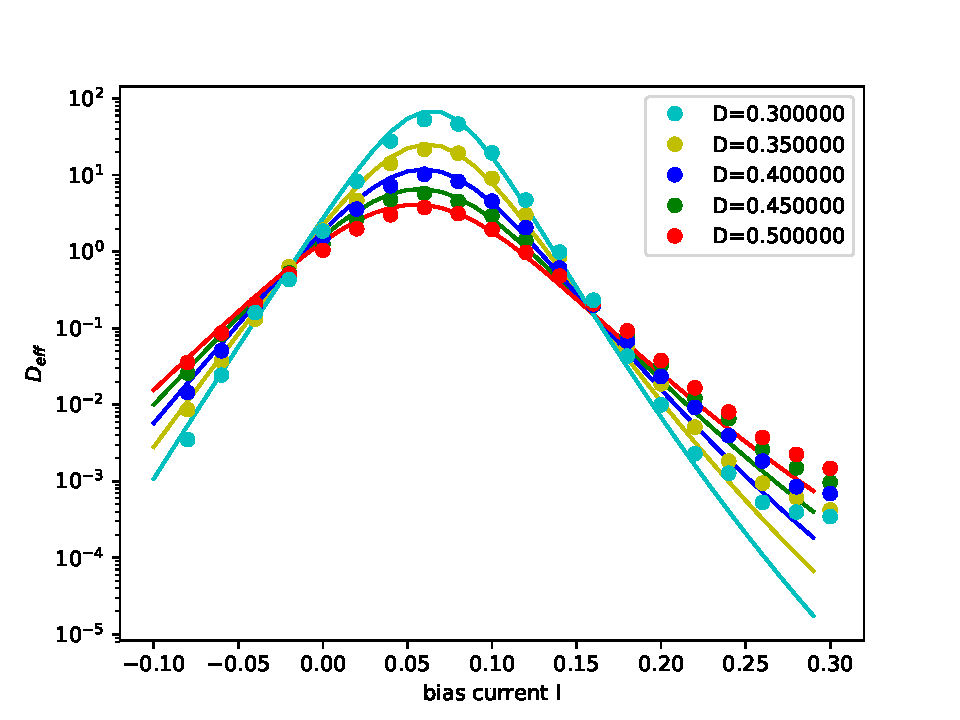
\includegraphics[scale=0.9]{dcompdfqnewrealfast11jjem2shrealfast19jjem2st.pdf}
	\caption{Vergleich Diffusionskoeffizient und verallgemeinerte Zwei-Zustands-Theorie mit quadratischen Barrieren}
	\label{dcompqua}
\end{figure}
Daher ist es auch nicht überraschend, dass das SNR mit dem allgemeinen Zwei-Zustands-Modell gut angenähert wird:
\begin{figure}[H]
	\centering
	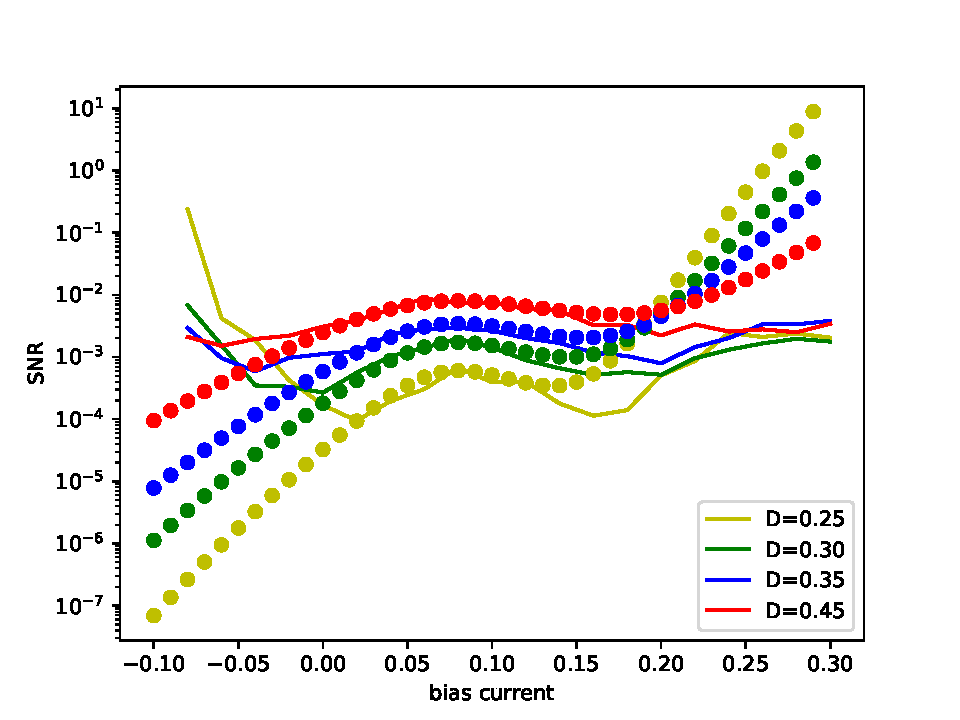
\includegraphics[scale=0.9]{snrautoreal13a25snr.pdf}
	\caption{Vergleich SNR mit der verallgemeinerten Zwei-Zustands-Theorie mit quadratischen Barrieren}
	\label{snrtwo}
\end{figure}
\section{Einfluss der Parameter}
\begin{figure}[H]
	\centering
	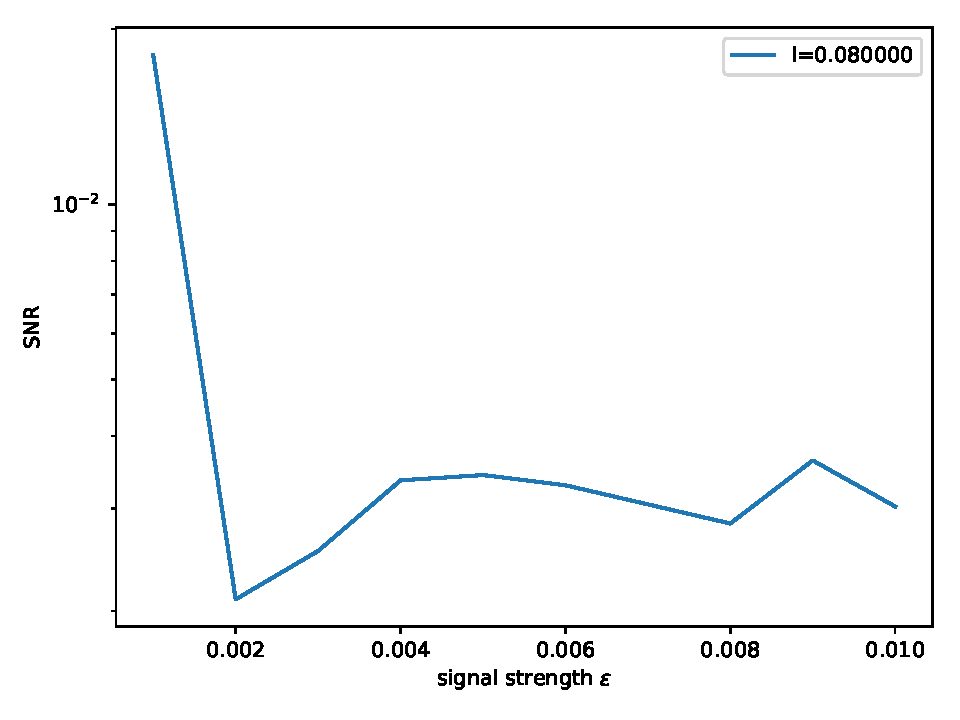
\includegraphics[scale=0.9]{snrepsautorealdrange6aem2.pdf}
	\caption{Abhängigkeit des gemessenen SNR von der Signalstärke}
	\label{eps}
\end{figure}
\end{document}